\documentclass{homework}

\title{Problem Set 4}
\author{Kevin Evans}
\studentid{11571810}
\date{February 28, 2021}
\setclass{Physics}{463}
\usepackage{amssymb}
\usepackage{mathtools}
\usepackage{graphicx}
\usepackage{amsthm}
\usepackage{amsmath}
\usepackage{slashed}
\usepackage{boldline}
\usepackage{physics}
\usepackage{tcolorbox}
\usepackage[inter-unit-product =\cdot]{siunitx}

\usepackage[makeroom]{cancel}
\usepackage{booktabs}
\usepackage{multirow}

\usepackage{times}
\usepackage{mhchem}
\usepackage{enumitem}
\usepackage[normalem]{ulem}
\usepackage{systeme}
\usepackage{tikz}
\usepackage{mathtools}
\usepackage{tabularx}
\usepackage{listings}


\newcommand{\fm}{\femto\meter}
\newcommand{\solution}{	\vspace{1em} \textit{Solution.} \quad }

\begin{document}
	\maketitle
	\begin{enumerate}
		\item % 4.1
			\textbf{\textit{Monatomic linear lattice.}} Consider a longitudinal wave 
				$$u_s = u \cos(\omega t - sKa)$$
				which propagates in a monatomic linear lattice of atoms of mass $M$, spacing $a$, and nearest-neighbor interaction $C$.
				
				\begin{enumerate}
					\item Show that the total energy of the wave is $$E=\frac{1}{2} M \sum_s \left(\dv{u_s}{t}\right)^2 + \frac{1}{2} C \sum_s (u_s - u_{s+1})^2,$$
					where $s$ runs over all atoms.
					
						\solution For an atom, the classical kinetic energy is given by \begin{align*}
							T_s & = \frac{1}{2} M \dot{u}_s^2.
							\intertext{Then for all atoms $s$, all the kinetic energies contribute to the total}
							T & = \frac{1}{2} M \sum_s \left(\dv{u_s}{t}\right)^2.
						\end{align*}
						The potential energy for a spring is \begin{align*}
							U_s & = \frac{1}{2} C (\Delta u)^2 \\
								& = \frac{1}{2} C \left(u_s - u_{s+1}\right)^2.
						\end{align*}
						(I don't really understand why $\Delta u$ is the difference between neighboring atoms, instead of the displacement from $u_s - 0 = u_s$. Isn't it normally the total displacement from equilibrium of the specific spring?)
						
						Combining these, the total energy is \begin{align*}
							E & = T + U \\
								& =\frac{1}{2} M \sum_s \left(\dv{u_s}{t}\right)^2 + \frac{1}{2} C \sum_s (u_s - u_{s+1})^2
						\end{align*}
					\item By substitution of $u_s$ in this expression, show that the time-average total per atom is $$\frac{1}{4} M \omega^2 u^2 + \frac{1}{2} C \left(1 - \cos Ka\right)u^2 = \frac{1}{2} M \omega^2 u^2,$$
					where in the last step, we have used the dispersion relation (9) for this problem.
					
						\solution For the kinetic term, \begin{align*}
							\dot{u}_s & = -\omega \sin(\dots),
							\intertext{As $\expval{\sin[2](\dots)} = 1/2$,}
							\implies \expval{\left(\dot{u}_s\right)^2} & = \frac{ \omega^2 u^2 }{2}. \\
							\implies \expval{T} & = \frac{1}{4} M \omega^2 u^2.
						\end{align*}
						Next, for the potential term,  \begin{align*}
							U_s & = \frac{u}{2} C \left(
								\cos(\omega t - sKa)
								- \cos(\omega t - sKa - Ka)
							\right)^2 \\
							\intertext{I'm not sure how to simplify the difference of cosines, so I'll just assume it'll simplify to the answer given in the question...}
							\expval{U_s} & = \frac{1}{2} C \left(1 - \cos Ka\right) u^2.
							\intertext{Removing the sums (since it's per atom), the time-average total energy per atom is }
							\expval{E} & = \expval{T} + \expval{U} \\
								& = \frac{1}{4} M \omega^2 u^2 + \frac{1}{2} C \left(1 - \cos Ka\right) u^2. \qed
						\end{align*}
				\end{enumerate}
			
		\item % 4.3
			\textbf{\textit{Basis of two unlike atoms.}} For the problem treated by (18) to (26), find the amplitude of the ratios $u/v$ for the two branches at $K_\mathrm{max} = \pi / a$. Show that at this value of $K$, the two lattices act as if decoupled: one lattice remains at rest while the other lattice moves.
			
			\solution At $Ka = \pi$ and using (20), the coupled equations become \begin{align*}
				- \omega^2 M_1 u & = Cv \left[1 + \underbrace{ \exp(-i \pi) }_{-1}\right] - 2 Cu = -2Cu ; \\
				- \omega^2 M_2 v & = Cu \left[\underbrace{\exp(i \pi)}_{-1} + 1\right] - 2 Cv = - 2Cv.
			\end{align*}
			These coupled equations now become decoupled, as there is no $v$-dependence in $u$, and vice-versa. So, the equations of motion will now look something like \begin{align*}
				u(t) & \approx u\exp(\sqrt{2C / M_1}t) ;\\
				v(t) & \approx v\exp(\sqrt{2C / M_2}t) .
			\end{align*}
		
		\pagebreak
		
		\item % 4.5
			\textbf{\textit{Diatomic chain.}} Consider the normal modes of a linear chain in which the force constants between nearest-neighbor atoms are alternatively $C$ and $10C$. Let the masses be equal, and let the nearest-neighbor separation be $a/2$. Find $\omega(K)$ at $K=0$ and $K=\pi/a$. Sketch in the dispersion relation by eye. This problem simulates a crystal of diatomic molecules such as \ce{H2}.
			
			\solution With reference to Figure 9 of Kittel, we can let $u_s$'s spring constant be $C$ and $v_s$'s spring constant be $10C$. Then we can rewrite (18) as \begin{align*}
				M \ddot{u}_s & = C(v_s + 10 v_{s-1} - u_s - 10u_s) ; \\
				M \ddot{v}_s & = C(u_{s+1} + 10 u_s - v_s - 10 v_s) .
			\end{align*}
			Using the ansatz (19), \begin{align*}
				\ddot{u}_s & = -\omega^2 u(s) ; \\
				\ddot{v}_s & = -\omega^2 v(s).
			\end{align*}
			Substituting this in, we find \begin{align*}
				-\omega^2 M u_s & = C \left( v_s + 10 v_{s-1} - u_s - 10 u_s\right) ; \\
				-\omega^2 M v_s & = C \left( u_{s+1} + 10 u_s - v_s - 10v_s\right).
				\intertext{Adding in the phase difference of $Ka$ on the $s\pm 1$ terms,} 
				-\omega^2 M u_s & = C \left( v_s + 10 \exp(-iKa) v_s - u_s - 10 u_s\right) ; \\
				-\omega^2 M v_s & = C \left( \exp(iKa) u_s + 10 u_s - v_s - 10v_s\right).
			\end{align*} 
			In matrix form, we can equate the determinate of the system to zero, \begin{align*}
				\begin{vmatrix}
					11C -M\omega^2  & -C\left[1 + 10 \exp(-iKa) \right] \\
					-C \left(10 + \exp(iKa) \right) & 11C - M \omega^2
				\end{vmatrix} & = 0,
				\intertext{or}
				\left(11C - M \omega^2\right)^2 - C^2 (1 + 10 \exp(-iKa))(10 + \exp(iKa))& = 0.
			\end{align*}
			For $Ka = 0$, \begin{align*}
				(11 C - M \omega^2)^2 & = C^2 (1 + 10)(10 + 1)  \\
				\omega^2(Ka = 0)  & \approxeq \frac{1}{M} \left(\sqrt{11^2C^2} + 11C\right) \\
					& \approxeq \frac{1}{M} \left(22C\right).
			\end{align*}
			For the zone boundary $Ka = \pi$, \begin{align*}
				(11 C - M \omega^2)^2 & = C^2(1 - 10)(10 - 1)  \\
				(11 C - M \omega^2) & = \pm 9C\\
				\omega^2(Ka = \pm \pi) & \approxeq \begin{cases}
					\frac{1}{M}  \left(20C\right) \\
					\frac{1}{M} \left(2C\right).
				\end{cases}
			\end{align*}
			
			\pagebreak
			Sketching this out, 
			\begin{center}
				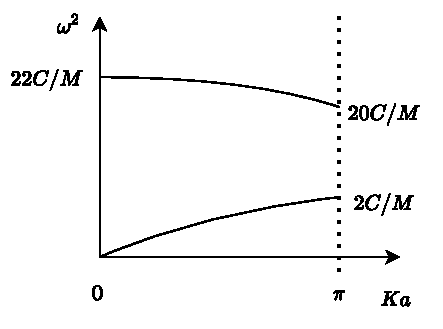
\includegraphics{plot.drawio.pdf}
			\end{center}

		
	\end{enumerate}
\end{document}